% Automatically generated by go_latex.py
%
\renewcommand{\one}{real_wood-knotty}
\renewcommand{\two}{real_cards-blue}

\setlength{\resLen}{0.558in}
\begin{figure*}[t]
    \centering
    \small
    \addtolength{\tabcolsep}{-4pt}
    \begin{tabular}{rrlrcc@{\hspace{2\tabcolsep}}lrcc}
    	&
        & \multicolumn{2}{c}{\textbf{SVBRDF maps}} & \multicolumn{2}{c}{\textbf{Novel views}}
        & \multicolumn{2}{c}{\textbf{SVBRDF maps}} & \multicolumn{2}{c}{\textbf{Novel views}}
        \\[2pt]
        & &
        & \raisebox{0.40\resLen}{\rotatebox[origin=c]{90}{\scriptsize GT}} &
        \includegraphics[height=\resLen]{results/refine/\one/ref/rendered_nov_1.jpg} &
        \includegraphics[height=\resLen]{results/refine/\one/ref/rendered_nov_2.jpg} &
        & \raisebox{0.40\resLen}{\rotatebox[origin=c]{90}{\scriptsize GT}} &
        \includegraphics[height=\resLen]{results/refine/\two/ref/rendered_nov_1.jpg} &
        \includegraphics[height=\resLen]{results/refine/\two/ref/rendered_nov_2.jpg}
        \\[-1pt]
        & &
        \textit{~~wood-knotty} & &
        \includegraphics[height=0.5\resLen]{results/refine/\one/ref/rendered_nov_1_zoom.jpg} &
        
\includegraphics[height=0.5\resLen]{results/refine/\one/ref/rendered_nov_2_zoom.jpg} &
        \textit{~~cards-blue} & &
        \includegraphics[height=0.5\resLen]{results/refine/\two/ref/rendered_nov_1_zoom.jpg} &
        
\includegraphics[height=0.5\resLen]{results/refine/\two/ref/rendered_nov_2_zoom.jpg}
        \\[2pt]
        \multirow{4}{*}[-1.4em]{\rotatebox[origin=c]{90}{\scriptsize\bfseries No refinement}} &
        \raisebox{0.40\resLen}{\rotatebox[origin=c]{90}{\scriptsize Ours (NR)}} &
        \multicolumn{2}{c}{\includegraphics[height=\resLen]{results/refine/\one/ours/tex.jpg}} &
        \includegraphics[height=\resLen]{results/refine/\one/ours/rendered_nov_1.jpg} &
        \includegraphics[height=\resLen]{results/refine/\one/ours/rendered_nov_2.jpg} &
        \multicolumn{2}{c}{\includegraphics[height=\resLen]{results/refine/\two/ours/tex.jpg}} &
        \includegraphics[height=\resLen]{results/refine/\two/ours/rendered_nov_1.jpg} &
        \includegraphics[height=\resLen]{results/refine/\two/ours/rendered_nov_2.jpg}
        \\[-1pt]
        & &
        \multicolumn{2}{c}{
\includegraphics[height=0.5\resLen]{results/refine/\one/ours/tex_zoom.jpg}} &
        \includegraphics[height=0.5\resLen]{results/refine/\one/ours/rendered_nov_1_zoom.jpg} &
        
\includegraphics[height=0.5\resLen]{results/refine/\one/ours/rendered_nov_2_zoom.jpg} &
        \multicolumn{2}{c}{
\includegraphics[height=0.5\resLen]{results/refine/\two/ours/tex_zoom.jpg}} &
        \includegraphics[height=0.5\resLen]{results/refine/\two/ours/rendered_nov_1_zoom.jpg} &
        
\includegraphics[height=0.5\resLen]{results/refine/\two/ours/rendered_nov_2_zoom.jpg}
        \\[2pt]
        & \raisebox{0.40\resLen}{\rotatebox[origin=c]{90}{\scriptsize [Gao19]+ (NR)}} &
        \multicolumn{2}{c}{\includegraphics[height=\resLen]{results/refine/\one/msra_egsr/tex.jpg}} &
        \includegraphics[height=\resLen]{results/refine/\one/msra_egsr/rendered_nov_1.jpg} &
        \includegraphics[height=\resLen]{results/refine/\one/msra_egsr/rendered_nov_2.jpg} &
        \multicolumn{2}{c}{\includegraphics[height=\resLen]{results/refine/\two/msra_egsr/tex.jpg}} &
        \includegraphics[height=\resLen]{results/refine/\two/msra_egsr/rendered_nov_1.jpg} &
        \includegraphics[height=\resLen]{results/refine/\two/msra_egsr/rendered_nov_2.jpg}
        \\[-1pt]
        & &
        \multicolumn{2}{c}{
\includegraphics[height=0.5\resLen]{results/refine/\one/msra_egsr/tex_zoom.jpg}} &
        \includegraphics[height=0.5\resLen]{results/refine/\one/msra_egsr/rendered_nov_1_zoom.jpg} &
        
\includegraphics[height=0.5\resLen]{results/refine/\one/msra_egsr/rendered_nov_2_zoom.jpg} &
        \multicolumn{2}{c}{
\includegraphics[height=0.5\resLen]{results/refine/\two/msra_egsr/tex_zoom.jpg}} &
        \includegraphics[height=0.5\resLen]{results/refine/\two/msra_egsr/rendered_nov_1_zoom.jpg} &
        
\includegraphics[height=0.5\resLen]{results/refine/\two/msra_egsr/rendered_nov_2_zoom.jpg}
        \\
        \hline\\[-8pt]
        \multirow{4}{*}[-1em]{\rotatebox[origin=c]{90}{\scriptsize\bfseries With refinement}} &
        \raisebox{0.40\resLen}{\rotatebox[origin=c]{90}{\scriptsize Ours}} &
		\multicolumn{2}{c}{\includegraphics[height=\resLen]{results/refine/\one/ours+/tex.jpg}} &
		\includegraphics[height=\resLen]{results/refine/\one/ours+/rendered_nov_1.jpg} &
		\includegraphics[height=\resLen]{results/refine/\one/ours+/rendered_nov_2.jpg} &
		\multicolumn{2}{c}{\includegraphics[height=\resLen]{results/refine/\two/ours+/tex.jpg}} &
		\includegraphics[height=\resLen]{results/refine/\two/ours+/rendered_nov_1.jpg} &
		\includegraphics[height=\resLen]{results/refine/\two/ours+/rendered_nov_2.jpg}
		\\[-1pt]
		& &
		\multicolumn{2}{c}{
\includegraphics[height=0.5\resLen]{results/refine/\one/ours+/tex_zoom.jpg}} &
		\includegraphics[height=0.5\resLen]{results/refine/\one/ours+/rendered_nov_1_zoom.jpg} &
		
\includegraphics[height=0.5\resLen]{results/refine/\one/ours+/rendered_nov_2_zoom.jpg} &
		\multicolumn{2}{c}{
\includegraphics[height=0.5\resLen]{results/refine/\two/ours+/tex_zoom.jpg}} &
		\includegraphics[height=0.5\resLen]{results/refine/\two/ours+/rendered_nov_1_zoom.jpg} &
		
\includegraphics[height=0.5\resLen]{results/refine/\two/ours+/rendered_nov_2_zoom.jpg}
		\\[2pt]
        & \raisebox{0.40\resLen}{\rotatebox[origin=c]{90}{\scriptsize [Gao19]+}} &
        \multicolumn{2}{c}{\includegraphics[height=\resLen]{results/refine/\one/msra+_egsr/tex.jpg}} &
        \includegraphics[height=\resLen]{results/refine/\one/msra+_egsr/rendered_nov_1.jpg} &
        \includegraphics[height=\resLen]{results/refine/\one/msra+_egsr/rendered_nov_2.jpg} &
        \multicolumn{2}{c}{\includegraphics[height=\resLen]{results/refine/\two/msra+_egsr/tex.jpg}} &
        \includegraphics[height=\resLen]{results/refine/\two/msra+_egsr/rendered_nov_1.jpg} &
        \includegraphics[height=\resLen]{results/refine/\two/msra+_egsr/rendered_nov_2.jpg}
        \\[-1pt]
        & &
        \multicolumn{2}{c}{\includegraphics[height=0.5\resLen]{results/refine/\one/msra+_egsr/tex_zoom.jpg}} &
        \includegraphics[height=0.5\resLen]{results/refine/\one/msra+_egsr/rendered_nov_1_zoom.jpg} &
        \includegraphics[height=0.5\resLen]{results/refine/\one/msra+_egsr/rendered_nov_2_zoom.jpg} &
        \multicolumn{2}{c}{\includegraphics[height=0.5\resLen]{results/refine/\two/msra+_egsr/tex_zoom.jpg}} &
        \includegraphics[height=0.5\resLen]{results/refine/\two/msra+_egsr/rendered_nov_1_zoom.jpg} &
        \includegraphics[height=0.5\resLen]{results/refine/\two/msra+_egsr/rendered_nov_2_zoom.jpg}
    \end{tabular}
    \caption{\label{fig:refine}
        \textbf{Per-pixel post-refinement.} Unlike Gao's method, post-refinement via per-pixel optimization makes less of a difference in our method.
        Without post-refinement, [Gao19]+ (i.e., Gao's method initialized with Deschaintre's~\shortcite{Deschaintre2019} direct predictions) usually produces blurry results, as shown in the row marked as ``[Gao19]+ (NR)''.
        Our method, on the contrary, does not rely nearly as heavily on post-refinement: Without it, our results are already quite sharp (see ``Ours (NR)''), thanks to the generative power of our MaterialGAN.
        A zoomed-in version is attached below each SVBRDF map and novel-view image.
    }
\end{figure*}
